\documentclass[12pt]{article}

%\usepackage{amsmath} % Advanced math typesetting
\usepackage{CJK} % chinese package
%\usepackage{CJKutf8} % chinese package
\usepackage{enumerate} % list by number
\usepackage{graphicx} % Add pictures to your document
\graphicspath{ {E:/[3-2]Project/document/Mod_c.png} }
\graphicspath{ {E:/[3-2]Project/document/Mod-1.png} }
\graphicspath{ {E:/[3-2]Project/document/Mod-2.png} }
\usepackage[a4paper,left=3cm,right=2cm,top=2.5cm,bottom=2.5cm]{geometry} % change font type % reference: https://www.sharelatex.com/learn/Font_typefaces
\usepackage{hyperref} % Add a link to your document
\usepackage[utf8]{inputenc} % Unicode support (Umlauts etc.)
%\usepackage{listings} % Source code formatting and highlighting
\usepackage[normalem]{ulem} % strikeout line, reference http://tex.stackexchange.com/questions/23711/strikethrough-text

\title{Project Purpose}
\date{\today}
\author{Hu Ting Kai}

\newcommand\tab[1][1cm]{\hspace*{#1}}

\begin{document}
	\maketitle
	\tableofcontents
	\newpage
	
	\begin{CJK}{UTF8}{bkai}
	\section{Introduction}
	\tab This project will develop a mod for Minecraft(including forge). By developing graphic user interface and convenient crafting recipe, the mod will be interesting, diversified design. This mod will make Minecraft more funny and more ways to play.
		\subsection{Research motivation}
		\tab Since I knew and started playing Minecraft about five years ago, Minecraft, the sandbox game, inspired me to do the similar things like this game, creative, logical and attractive, then I knew this is called programming. After learning basic knowledge about programming, I decide to go back to the beginning, and that is Minecraft.
		\subsection{Research purpose}
		\tab Learn how to develop a mod in specific version of Minecraft, and build a mod for all platform users, including Windows, MacOS and Linux. %\sout{And also I have an execution to play Minecraft while doing project.}
		\subsection{Research range}
		\begin{enumerate}[i.]
			\item Java SE.
			\item Minecraft source code, if I can get it.
			\item Minecraft forge source code.
		\end{enumerate}
		\tab etc. If I can figure out more.
	\section{System function}
	\tab Objective: Overwatch, a game a team-based multiplayer first-person shooter video game developed and published by Blizzard Entertainment.\\
	\begin{enumerate}[i.]
		\item Characters' costumes: build all characters' costume and reference to each specific recipe.
		\item Characters' weapons: build all characters' weapons and their special ability such as speed decreasing, power up, etc.
		\item Mob: like zombies and creepers, the mod's mobs will spawn when night coming, like original Minecraft mobs.
		\item (Optional, if I can still do) Original game scene: build part of building in the Minecraft map spawned randomly when map created.
	\end{enumerate}
	\section{Development System environment}
	\begin{enumerate}[i.]
		\item Windows 7 professional
		\item JDK 1.8+
		\item Minecraft 1.10.*
		\item Minecraft forge 1.10.*
	\end{enumerate}
	\section{Excepted schedule}
	\begin{figure}[h]
	%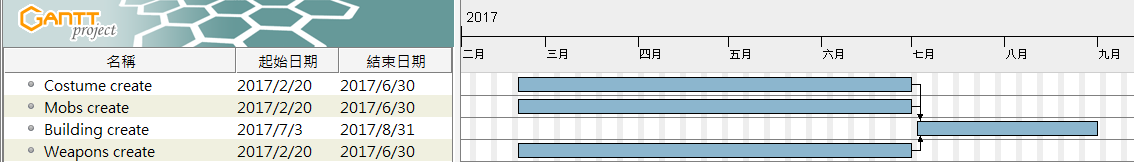
\includegraphics[width=\textwidth]{Mod_c}
	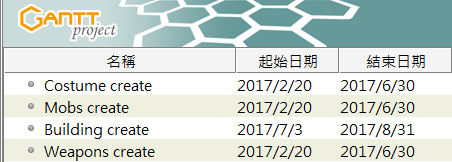
\includegraphics[width=\textwidth]{Mod-1}\\
	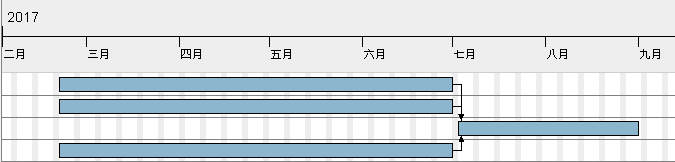
\includegraphics[width=\textwidth]{Mod-2}
	\end{figure}
	\section{Excepted result}
	\tab A .jar file that contain mod that Minecraft 1.10.* with forge can load for all cross-platform user.
	\newpage
	\section*{References}
	\url{http://minecraft.gamepedia.com/Mods/Creating_mods}\\
	\url{http://www.minecraftforum.net/forums/mapping-and-modding/mapping-and-modding-tutorials/2718726-list-of-minecraft-1-10-x-modding-tutorials}\\
	\url{https://bedrockminer.jimdo.com/modding-tutorials}\\
	\end{CJK}
\end{document}